\chapter{Plataforma de desarrollo}
\label{cap:capitulo3}

\begin{flushright}
\begin{minipage}[]{10cm}
\emph{Un buen artesano no se separa nunca de sus herramientas, las conoce y las elige con sabiduría.}\\
\end{minipage}\\

Leonardo da Vinci\\
\end{flushright}

\vspace{1cm}

%Escribe aquí un párrafo explicando brevemente lo que vas a contar en este capítulo. En este capítulo, explica qué has usado a nivel hardware y software para poder desarrollar tu trabajo: librerías, sistemas operativos, plataformas, entornos de desarrollo, etc.

En este capítulo describe la infraestructura, tanto de hardware como de
software, utilizada como base para el desarrollo y ejecución de los sistemas
robóticos que se explicarán más adelante.

\section{Hardware}
\label{sec:hardware}
% Portatil, raspberry, router, T2, T4 y explicacion ligera de sus componentes.

Como se ha detallado en el Capítulo \ref{cap:capitulo1}, el \textit{hardware}
constituye la infraestructura fundamental de los robots, definiendo sus
capacidades operativas.
Estas capacidades están intrínsecamente ligadas a los componentes físicos del
robot, lo que implica que la disponibilidad y calidad del \textit{hardware} son
críticas para ejecutar cualquier tarea.
Por ejemplo, la ausencia de un sistema de agarre adecuado o la limitación en su
fuerza o precisión pueden comprometer la ejecución correcta de una tarea de
\textit{pick and place}.
\\

En nuestro caso, hemos utilizado plataformas robóticas como los famosos robots
de la familia Turtlebot\footnote{\url{https://www.turtlebot.com/about/}}, en
concreto los modelos 2 y 4 \textit{Lite}, que se pueden apreciar en la Figura
\ref{fig:turtlebots}, debido a su naturaleza móvil y barata, y a su
disponibilidad en el laboratorio.
\\

\begin{figure} [h!]
  \begin{center}
    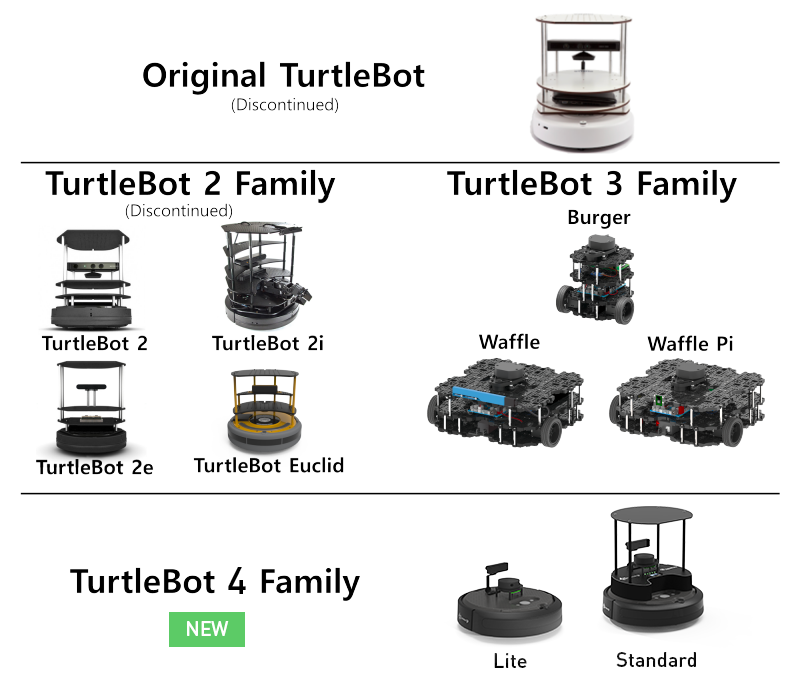
\includegraphics[width=11cm]{figs/turtlebot_family}
  \end{center}
  \caption{Modelos del robot Turtlebot \cite{turtlebot4}}
  \label{fig:turtlebots}
\end{figure}\

\subsection{Turtlebot 2}
\label{sec:turtlebot2}

En concreto, el robot Turtlebot
2\footnote{\url{https://www.turtlebot.com/turtlebot2/}} se fundamenta en la base
\textit{Kobuki}, que dispone de los sensores necesarios para una navegación
robusta, como puede ser la IMU o Unidad de Medida Inercial, para las
correcciones en los datos de odometría y un \textit{bumper} o sensor de
colisiones.
La base \textit{Kobuki} también dispone de una batería que dota al robot de
cierta autonomía.
Asimismo, dispone de actuadores que le permiten llevar a cabo dicha navegación,
como son los motores y otros que le permiten transmitir información de manera
visual o auditiva, como los LEDs, y el \textit{buzzer}, con capacidad de
reproducir varios sonidos.
\\

\begin{figure} [h!]
  \begin{center}
    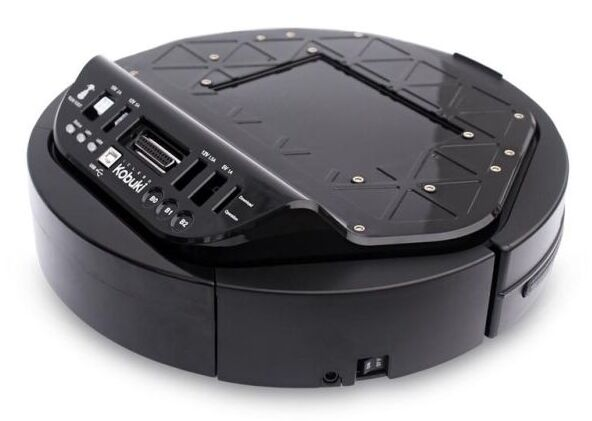
\includegraphics[width=6cm]{figs/kobuki_base}
  \end{center}
  \caption{Base Kobuki \cite{kobuki_base}}
  \label{fig:base_kobuki}
\end{figure}\

Aparte de los componentes de la base, el robot cuenta con una estructura de
madera soportada por barras de aluminio que permite apoyar un ordenador
portátil a modo de ordenador de a bordo, y sensores externos, cuyos modelos
pueden variar dependiendo del robot utilizado en cada momento, ya que se
disponen de varias configuraciones de los mismos en el laboratorio, sin afectar
a la compatibilidad.
Dichos sensores son: un LIDAR para la detección de obstáculos (modelos
RPLIDAR\footnote{\url{https://www.slamtec.ai/product/slamtec-rplidar-s2/?gad_source=1&gclid=CjwKCAjwrIixBhBbEiwACEqDJdjBNB-VeyXLm1hxO33F5wKfJLRu6KRyC1aa4NfaTWvre8dR0scc8xoCMq8QAvD_BwE}}
A1 o A2), y una cámara RGBD, de color RGB y profundidad (modelos
Orbbec\footnote{\url{https://www.orbbec.com/}} Astra o
Asus\footnote{\url{https://www.asus.com/es/}} Xtion).
Este último sensor aporta un gran potencial debido a su versatilidad en cuanto a
la detección se refiere.
Se puede ver una imagen del modelo en la Figura \ref{fig:turtlebot2}.
\\

\begin{figure} [h!]
  \begin{center}
    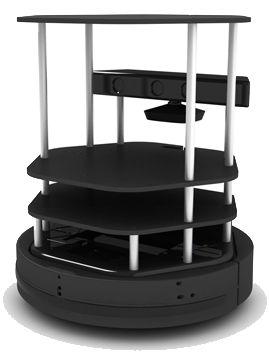
\includegraphics[width=6cm]{figs/turtlebot2}
  \end{center}
  \caption{Turtlebot 2 \cite{turtlebot4}}
  \label{fig:turtlebot2}
\end{figure}\


\subsection{Turtlebot 4}
\label{sec:turtlebot4}

Por su parte, el robot Turtlebot 4\footnote{\url{https://www.turtlebot.com/}}
\textit{Lite} utilizado es bastante parecido al anterior en cuanto a los
sensores de la base se refiere, correspondiendo esta vez con el modelo Create 3
de iRobot\footnote{
\url{https://www.irobot.es/es_ES/roomba.html?gad_source=1&gclid=CjwKCAjwrIixBhBbEiwACEqDJcM6GMOs9Ew0S98K9IJvOaBGm30dR6D1pk5T09dpqwcvNVTaYr7ZTBoC3HgQAvD_BwE}}
que, a efectos prácticos, es una aspiradora robótica sin la aspiradora ni las
escobillas que las caracterizan.
\\

Este robot también añade un sensor LIDAR y una cámara RGBD, que, en el caso de
nuestro laboratorio, son los modelos \textit{RPLIDAR-S2} y \textit{Oak-D-Pro}
respectivamente, sustituyendo a los modelos originales \textit{RPLIDAR-A1} y
\textit{Oak-D-Lite}.
A diferencia de su versión estándar y del anterior robot, este no tiene una
estructura de soporte, por lo que el ordenador de a bordo es una Raspberry
Pi 4 Model B\footnote{
\url{https://www.raspberrypi.com/products/raspberry-pi-4-model-b/}}, como la
mostrada anteriormente en la Figura \ref{fig:raspberry_pi}, que en nuestro caso
tiene 8Gb de RAM, aunque en el modelo original es de 4Gb.
Se puede ver una imagen del modelo de dicho robot en la Figura
\ref{fig:turtlebot4}.
\\

\begin{figure} [h!]
  \begin{center}
    \includegraphics[width=8cm]{figs/turtlebot4}
  \end{center}
  \caption{Turtlebot 4 \textit{Lite} (izquierda) y Standard (derecha) \cite{turtlebot4}}
  \label{fig:turtlebot4}
\end{figure}\


\subsection{Ordenadores de a bordo}
\label{sec:a_bordo}

Como ya se ha presentado en la Sección \ref{sec:turtlebot2}, para comandar
órdenes al robot se necesita un ordenador de a bordo.
En nuestro caso se ha utilizado un ordenador portátil, de la marca HP, modelo
\textit{ProBook 450 G6}\footnote{
\url{https://support.hp.com/es-es/document/c06195762}}.
\\

\begin{figure} [h!]
  \begin{center}
    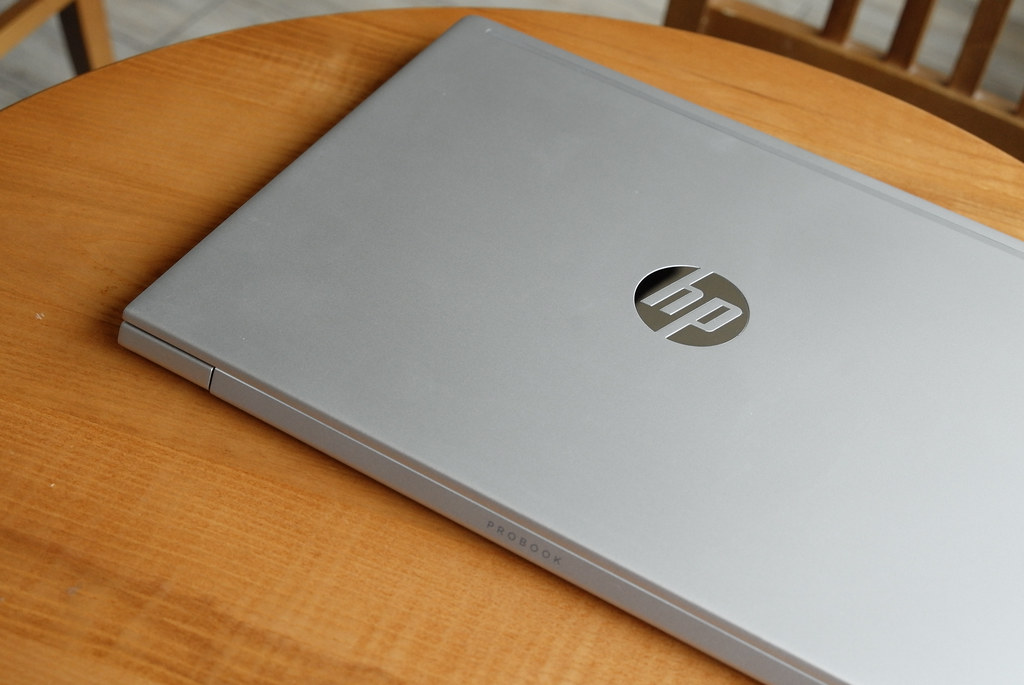
\includegraphics[width=8cm]{figs/hp_probook}
  \end{center}
  \caption{Ordenador portátil HP, modelo ProBook 450 G6 \cite{hp_probook}}
  \label{fig:hp_probook}
\end{figure}\

Para algunas pruebas también se añadió una Raspberry Pi 4 Model B, de 4Gb de
RAM, como ordenador de a bordo de un robot Turtlebot 2.
\\

\begin{figure} [h!]
  \begin{center}
    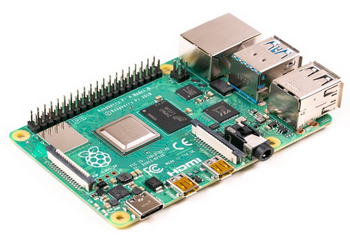
\includegraphics[width=8cm]{figs/raspberry_pi_4b}
  \end{center}
  \caption{Raspberry Pi 4, modelo B \cite{raspberry_pi_4b}}
  \label{fig:raspberry_pi}
\end{figure}\


\subsection{Ordenador principal}
\label{sec:ordenador_principal}

Para llevar a cabo este trabajo se precisó de la utilización de un ordenador con
la suficiente capacidad tanto de desarrollar el \textit{software}, como de
llevar a cabo las pruebas del mismo, ejecutando los resultados tanto en un
entorno simulado como en uno real.
Este ordenador también se corresponde con el portátil HP mencionado en la
Sección \ref{sec:a_bordo}.
\\

En cuanto a las pruebas realizadas con robots reales, el uso de este mismo
componente a modo de ordenador principal o centralizado también fue necesario.
Este ordenador portátil es el \textit{hardware} en el que se albergó toda la
capacidad de cómputo acerca de la toma de decisiones, así como el lugar de
ejecución del \textit{software} utilizado para la ejecución de la aplicación
robótica creada.
\\

\subsection{Router}
\label{sec:router}

La comunicación entre los distintos robots es una parte indispensable de este
trabajo, por lo que surge la necesidad de añadir un \textit{hardware} con la
capacidad de comunicar múltiples robots, en nuestro caso un router de la marca
ASUS, Modelo ROG Rapture
GT-AXE16000\footnote{\url{https://rog.asus.com/es/networking/rog-rapture-gt-axe16000-model/}}
sin necesidad de conexión a Internet, ya que se utiliza únicamente para la
comunicación local entre los distintos robots.
\\

\begin{figure} [h!]
  \begin{center}
    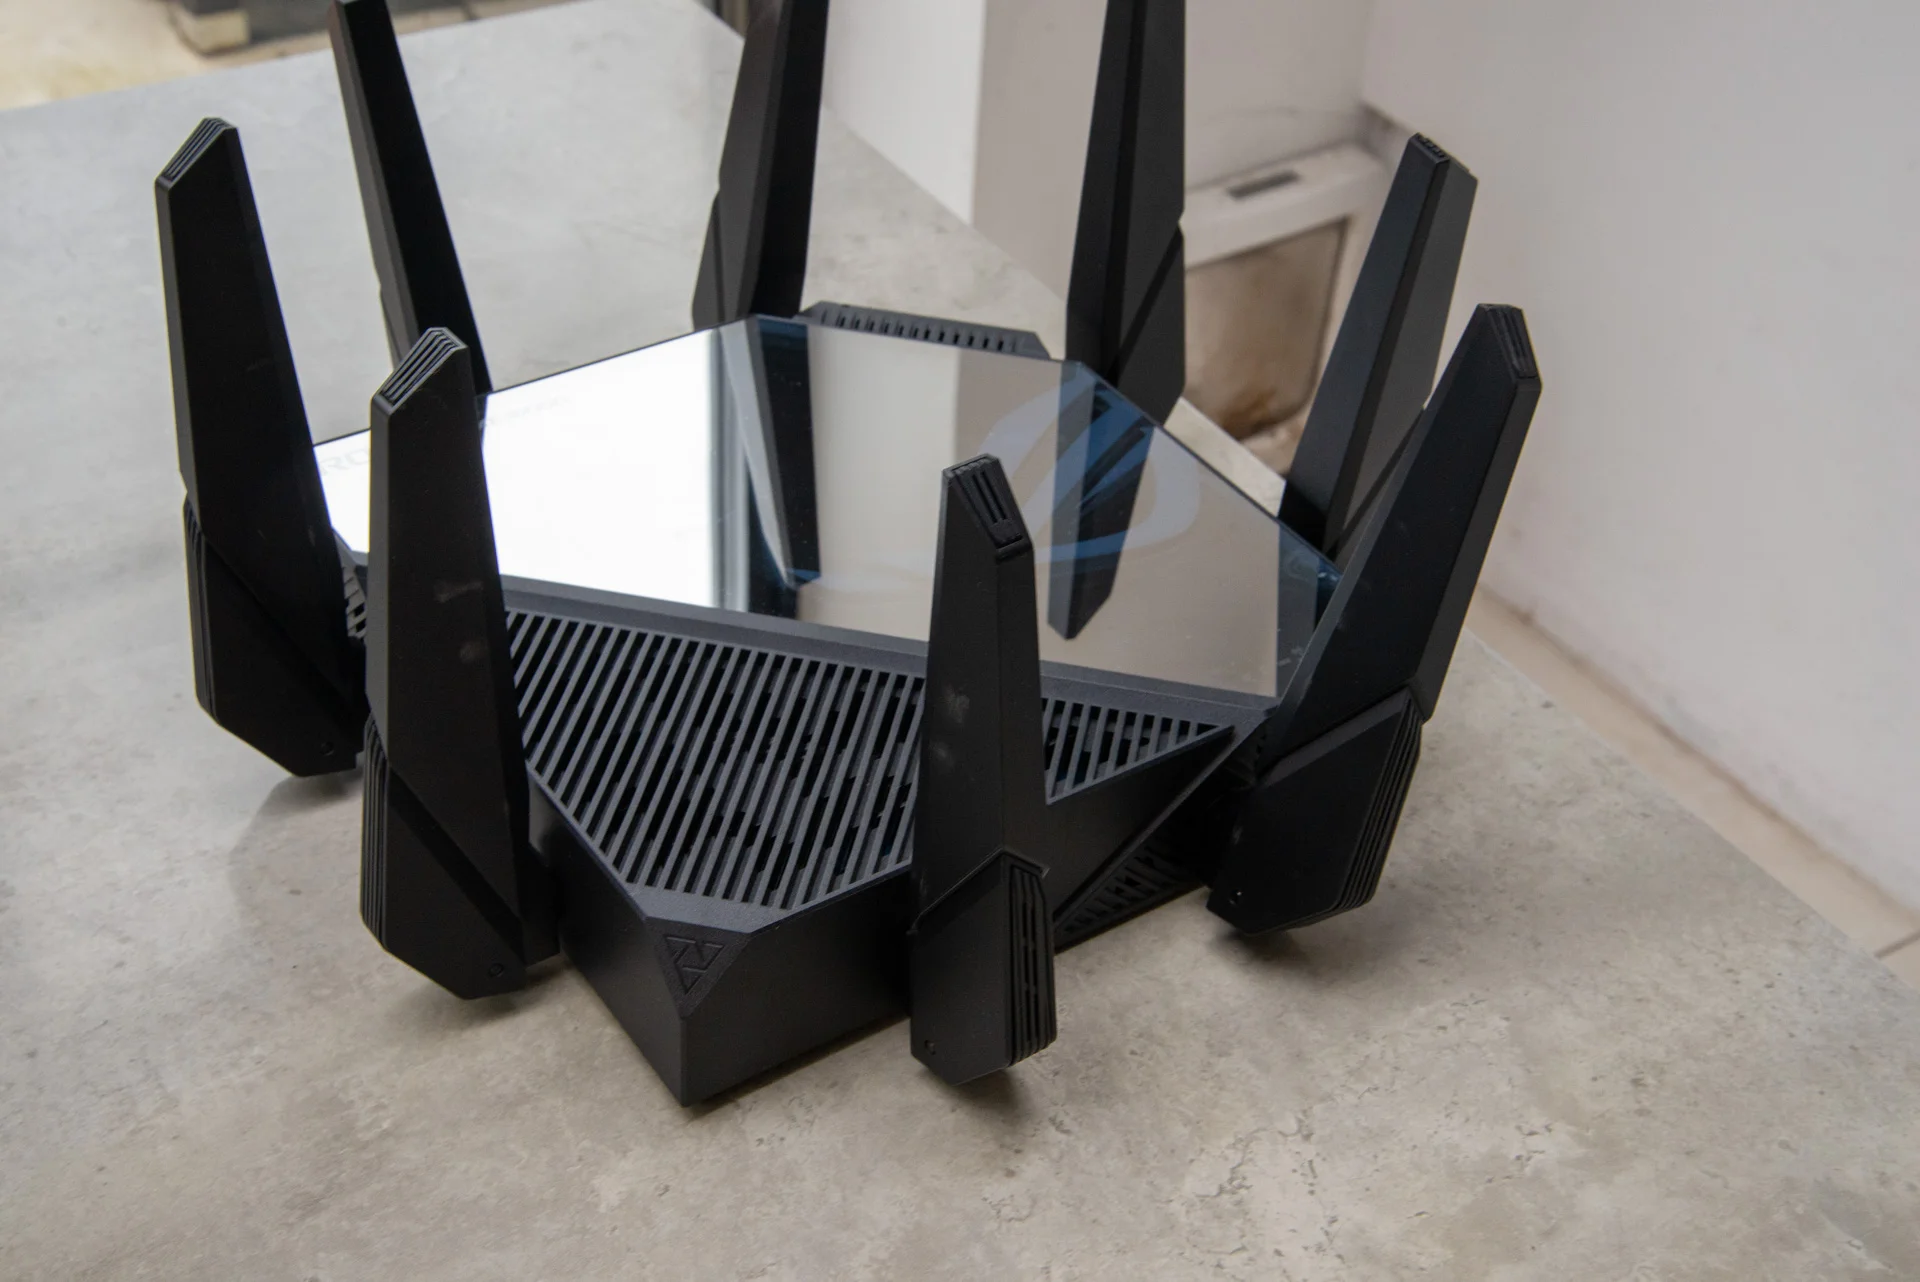
\includegraphics[width=8cm]{figs/asus_router}
  \end{center}
  \caption{Router ASUS, modelo ROG Rapture GT-AXE16000 \cite{asus_router}}
  \label{fig:asus_router}
\end{figure}\


\section{Software}
\label{sec:software}

El \textit{software} desempeña un papel crucial al convertir las capacidades del
\textit{hardware} en acciones concretas.
Es el encargado de emitir las instrucciones necesarias para que el robot, en
conjunto, funcione como un sistema inteligente capaz de llevar a cabo la tarea
definida.
En ausencia de una programación inteligente, el robot permanecerá como un
dispositivo inerte, con un potencial latente pero incapaz de realizar tareas de
manera autónoma.
\\

A continuación se explicarán las distintas herramientas \textit{software}
utilizadas, desde el sistema operativo, pasando por el lenguaje de programación
principal, hasta el \textit{middleware} robótico.
\\


\subsection{Sistema Operativo}
\label{sec:sistema_operativo}

El sistema operativo utilizado es Ubuntu en su versión 22.04 LTS (Long Term
Support o soporte a largo plazo).
Además, es una distribución basada en Debian GNU/Linux, que a su vez se basa en
el \textit{software} libre y de código abierto, lo que permite una mayor
participación de cualquier persona en su desarrollo, aumentando su robustez y
mejorando su soporte.
\\

Esta elección se fundamenta principalmente en la facilidad de uso y programación
con el mismo, así como la compatibilidad con el resto de programas utilizados.
La versión del sistema operativo utilizada coincide con la más nueva de soporte
a largo plazo en la fecha de realización de este proyecto.
\\


\subsection{Lenguaje de programación}
\label{sec:lenguaje_programacion}

El lenguaje de programación utilizado para el desarrollo del \textit{software}
de este trabajo, es \texttt{Python}, ya que debido a su sencillez de
programación y a su legibilidad de código, da lugar a un buen entorno para el
desarrollo de \textit{software} educativo, permitiendo una gran facilidad a la
hora de aprender, además de ser de código abierto, con las respectivas ventajas
que esto supone, explicadas en la Sección \ref{sec:sistema_operativo}.
\\

\texttt{Python} es un lenguaje de programación interpretado, lo que evita tener
que ser compilado, que suele conllevar un proceso tedioso para programadores
principiantes.
Además, se define como lenguaje de alto nivel, ya que soporta la programación
orientada a objetos (OOP), lo que también permite su escala en complejidad, si
así se requiriese.
\\

Este lenguaje ha tomado un gran impulso en los últimos años debido a su
popularidad, aunque cabe destacar que es un lenguaje sumamente lento en
comparación a otros más simples, y generalmente de más bajo nivel, como
\texttt{C}.
En concreto utilizaremos la versión 3 de este lenguaje debido a su
compatibilidad y a su relevancia actual.
\\

Este lenguaje de programación será usado directamente a la hora de programar
nuestro propio \textit{software}.
Además, otros lenguajes serán utilizados indirectamente por aplicaciones o nodos
externos.
Por ejemplo, \texttt{C++} será utilizado en algunos nodos de ROS2, mientras que
\texttt{Rust}, un lenguaje con una creciente popularidad y conocido por su
seguridad y rendimiento, además de su excelente gestión de la memoria, estará
presente en los programas relacionados con Zenoh.
\\

\subsection{Middleware Robótico}
\label{sec:middleware_robotico}

%Párrafo sobre ROS2
ROS2 es un \textit{middleware} robótico creado para abstraer al programador del
\textit{hardware} del robot, permitiendo una mayor atención en el desarrollo
\textit{software} del mismo.
Por todo ello, simplifica este proceso, sirviendo de herramienta tanto para la
programación o desarrollo, como para el uso o la ejecución del \textit{software}
en cuestión.
\\

En este \textit{middleware}, el código se divide en nodos ejecutables de manera
iterativa a una determinada frecuencia, que pueden comunicarse a través del
protocolo DDS, generalmente con la utilización de \textit{topics}, ya que dicho
protocolo basa su funcionamiento en un modelo de publicador/suscriptor, donde
los componentes del sistema se dividen en publicadores, responsables de enviar
datos, y suscriptores, encargados de recibirlos.
La comunicación se facilita mediante un \textit{broker} o intermediario, que
coordina la trasferencia de mensajes entre los nodos, permitiendo una
comunicación flexible y organizada en temas anteriormente llamados
\textit{topics}, y sin necesidad requerir que los publicadores y suscriptores
se conozcan directamente.
La librería cliente de ROS2 permite programar los nodos en \texttt{Python} o
\texttt{C++}, aunque la amplia comunidad ha desarrollado extraoficialmente el
equivalente en otros lenguajes como \texttt{Java}, \texttt{C}, \texttt{Rust} o
incluso \texttt{Android}, entre otros.
\\


\subsection{Simulación}
\label{sec:simulacion}

%Párrafo sobre Gazebo y lenguajes de marcado tipo XML como URDF/SDF
En cuanto a la simulación, el \textit{software} utilizado es Gazebo, un
simulador muy popular que permite la visualización de los robots y de los
entornos, gracias a su previa descripción, generalmente mediante un archivo con
formato XML (eXtensible Markup Language) o derivado, que pueden ser
URDF\footnote{\url{https://wiki.ros.org/urdf}} (Unified Robotics Description
Format) y SDF\footnote{\url{http://sdformat.org/}} (Simulation Description
Format) respectivamente.
Puede verse un ejemplo de simulación en la Figura \ref{fig:gazebo_sim}.
\\

\begin{figure} [h!]
  \begin{center}
    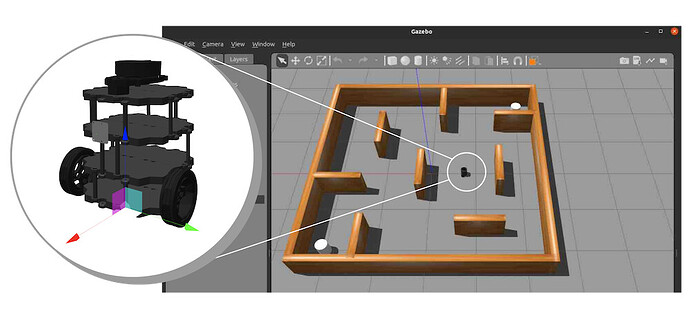
\includegraphics[width=10cm]{figs/gazebo_sim}
  \end{center}
  \caption{Gazebo simulando un robot Turtlebot 3 en un mundo virtual \cite{gazebo}}
  \label{fig:gazebo_sim}
\end{figure}\

Este simulador también permite la visualización de ciertos datos de sus sensores
si así se requiere, o de las partes o componentes de un robot gracias al archivo
de descripción del mismo, mencionado en el párrafo anterior.
Además permite el uso de \textit{plugins} que pueden añadir las funcionalidades
que sean necesarias.
\\


\subsection{Protocolos de comunicación}
\label{sec:protocolos_comunicacion}

%%% [Párrafo sobre ZettaScale y sus softwares utilizados]
En este ámbito, una de las empresas más importantes es ZettaScale
Technology\footnote{\url{https://www.zettascale.tech/}}, que ha tomado mucha
relevancia en los últimos años, ya que es responsable de una de las
implementaciones de \textit{middleware} de telecomunicaciones de DDS utilizado
en ROS2, llamado CycloneDDS\footnote{\url{https://cyclonedds.io/}}, y son los
desarrolladores de un reciente protocolo de comunicaciones llamado
Zenoh\footnote{\url{https://zenoh.io/}}, por sus siglas en inglés, Zero Overhead
Network Protocol, que ya cuenta con importantes clientes, como la NASA, debido a
las prestaciones que este ofrece, superando en la mayoría de casos a los
protocolos de su misma índole y que ya ha sido oficialmente seleccionado como el
próximo RMW (ROS \textit{Middleware} o \textit{Middleware} de comunicación de
ROS) de ROS2\footnote{
\url{https://discourse.ros.org/t/ros-2-alternative-middleware-report/33771}}.
El protocolo Zenoh, está basado en un modelo de publicador/suscriptor, así como
DDS, por lo que hacen una buena sinergia.
\\

Además de esto, poseen un potente \textit{framework} para la programación de
flujos de datos aún en desarrollo, llamado
Zenoh-Flow\footnote{\url{https://zenoh.io/blog/2023-02-10-zenoh-flow/}}, así
como un puente llamado
Zenoh-Bridge-DDS\footnote{\url{https://github.com/eclipse-zenoh/zenoh-plugin-dds}}
que hace las veces de traductor entre los protocolos DDS y Zenoh, lo que permite
la comunicación entre estos flujos de datos con nodos de ROS2, haciendo posible
la creación de aplicaciones robóticas en forma de flujos de datos, utilizando
nodos de ROS2 existentes, y fusionando de esta manera ambos campos.
\\

Es notable destacar el gran soporte que brinda esta empresa, que ayuda en gran
medida a resolver los problemas o dudas que puedan surgir durante el desarrollo o
despliegue de las aplicaciones.
\\

El protocolo de comunicaciones utilizado en el \textit{software} desarrollado en
este trabajo es Zenoh, que reduce en gran medida los bytes de la cabecera de los
mensajes, y ofrece mejores prestaciones en comparación con otros protocolos de
su misma índole, como se puede apreciar en la gráfica de la Figura
\ref{fig:zenoh_performance}, en la que se hicieron pruebas en varias máquinas,
con los protocolos Kafka, MQTT, CycloneDDS y distintas variantes de Zenoh,
siendo estas últimas las que mejores resultados obtuvieron.
\\

\begin{figure} [h!]
  \begin{center}
    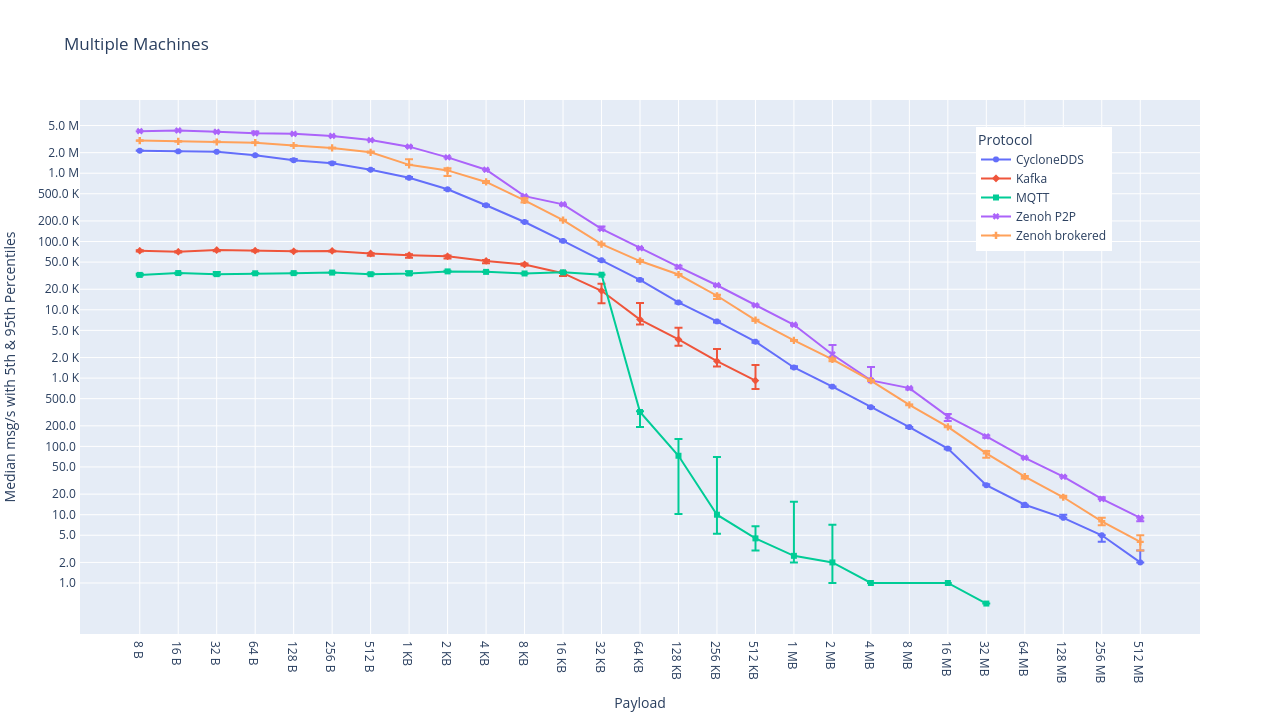
\includegraphics[width=15cm]{figs/zenoh_performance}
  \end{center}
  \caption{Rendimiento de distintos protocolos \cite{zenoh_performance}.}
  \label{fig:zenoh_performance}
\end{figure}\

En nuestro caso utilizaremos Zenoh-Flow para la programación de flujos de datos,
ya que tiene una API (Application Programming Interface) en \texttt{Python}, lo
que permite programarlos de manera sencilla, como se ha explicado en la Sección
\ref{sec:lenguaje_programacion}.
\\

También se utilizará DDS indirectamente en los nodos de ROS2 de los que se hará
uso, para los que utilizaremos la RMW de CycloneDDS, ya que es el que mejor
funciona con el software utilizado.
\\

Además, enlazaremos dichos nodos de ROS2 con nuestro flujo de datos mediante el
uso del Zenoh-Bridge-DDS, que nos permitirá traducir los mensajes de un
protocolo a otro en ambos sentidos, ya que Zenoh-Flow utiliza Zenoh para las
comunicaciones, mientras que ROS2 se comunica mediante DDS.
\\


\subsection{Visión Artificial}
\label{sec:vision_artificial}

Para la detección de objetos a partir de imágenes, ya sean generadas por una
cámara o creadas a partir de los datos de otros sensores, se ha utilizado una
reconocida librería de procesamiento de imágenes llamada OpenCV, disponible
tanto en \texttt{Python} como en \texttt{C++}.
\\

Este software permite, entre otras muchas cosas, el cambio entre distintos
espacios de color, entre los que se encuentran desde el formato RGB, pasando
por el formato GreyScale o escala de grises, que permite ahorrar memoria, o
detectar bordes, hasta el formato HSV (Hue, Saturation, Value), que permite,
entre otros muchos usos, trabajar con los colores en distintas intensidades de
luz, brindando así mejores resultados que con otros espacios de color.
Este espacio de color se ve representado en la Figura \ref{fig:hsv}.
\\

\begin{figure} [h!]
  \begin{center}
    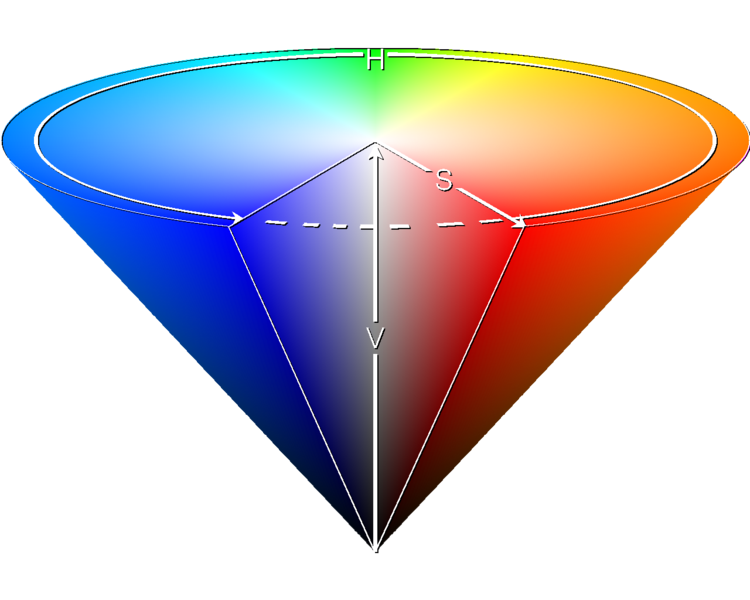
\includegraphics[width=6cm]{figs/hsv_cone}
  \end{center}
  \caption{Espacio de color HSV \cite{hsv_cone}}
  \label{fig:hsv}
\end{figure}\

Esta librería también permite distintos tipos de detecciones como pueden ser la
detección de rostros, bordes o contornos, o la detección de objetos mediante
aprendizaje profundo.
En nuestro caso, se han utilizado la detección de objetos mediante el uso de un
filtro de color aplicado a la imagen obtenida desde la cámara, y la detección de
bordes en conjunto con la posterior detección de círculos, en una imagen
generada a partir de los datos posicionales de un sensor LIDAR, como se explica
en la Sección \ref{sec:X} del capítulo de experimentos.
\\
%[TODO] añadir sección (\ref{sec:X}).

Esta librería también se apoya en otra, llamada Numpy, encargada de la
representación matemática eficiente de matrices, así como de operaciones
matemáticas entre ellas, ya que las imágenes a color, generalmente son matrices
tridimensionales, que albergan tres canales (RGB o HSV), cuyas columnas tienen
el tamaño de la longitud vertical de la imagen en píxeles, así como el tamaño de
las filas, corresponde con el ancho de la imagen, como se puede ver en la Figura
\ref{fig:rgb_mat}.
\\

\begin{figure} [h!]
  \begin{center}
    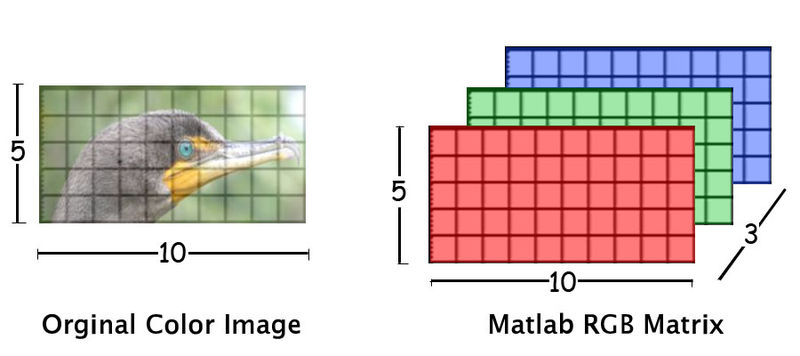
\includegraphics[width=10cm]{figs/rgb_matrix}
  \end{center}
  \caption{Representación de imagen RGB como matriz \cite{rgb_mat}}
  \label{fig:rgb_mat}
\end{figure}\


\subsection{Software de navegación}
\label{sec:navegacion}

El \textit{software} de navegación utilizado para trasladar los robots de una
posición a otra en el espacio se basa en los paquetes del conocido
\textit{stack} de Nav2\footnote{\url{https://navigation.ros.org/}}, que brinda
herramientas que solucionan la navegación del robot de manera bastante robusta y
precisa, gracias a un método de localización probabilístico basado en el
algoritmo de Montecarlo.
Este algoritmo consiste en distribuir una gran cantidad de puntos a lo largo del
mapa del entorno, que representan posibles ubicaciones del robot, y por tanto se
moverán de acuerdo al movimiento del mismo.
Además, tienen una probabilidad asociada basada en los datos de los sensores,
alrededor de la cual se desarrollará una nueva generación de partículas: se
partirá de las más probables añadiendo una variable de aleatoriedad y se
eliminarán las de menor probabilidad, acercándose de esta manera en cada
iteración a la posición real del robot, incluso en entornos altamente
simétricos.
\\


\subsection{Software matemático}
\label{sec:software_matematico}
%librerias Numpy, Math, y las transformadas de ROS2.

Para suplir la necesidad de realizar operaciones matemáticas de todo tipo, como
pueden ser las transformaciones entre espacios de coordenadas o entre ejes de
coordenadas, operaciones simples o complejas con grandes cantidades de números,
como matrices o imágenes, o cualquier otro tipo de operaciones, se han utilizado
tanto la librería Numpy como Math, dependiendo del tipo de operación, ya que
ambas son muy eficientes.
\\

Para operaciones de transformadas (TFs) de ROS2 entre dos \textit{frames},
utilizaremos las propias herramientas de ROS2, aunque no podremos utilizar
cualquiera, ya que la mayoría tienen la necesidad de correr en un nodo de ROS2
y no funcionan fuera del mismo, por lo que concretamente utilizaremos la
función del Código \ref{cod:code_tfs}.
Es por lo que se necesitará haber creado una suscripción previamente al
\textit{topic} de TFs del robot en cuestión.
\\

\begin{code}[h!]
  \begin{lstlisting}[language=Python]
    from builtin_interfaces.msg import Duration
    import tf2_ros, rclpy

    buffer_core = tf2_ros.BufferCore(Duration(sec=1, nanosec=0))
    buffer_core.lookup_transform_core(
      frame_id_1, frame_id_2, rclpy.time.Time()
      )
  \end{lstlisting}
  \caption[Función para calcular transformadas]{Función para calcular transformadas (TFs)}
  \label{cod:code_tfs}
\end{code}


\subsection{Visualización de datos}
\label{sec:visualizacion_datos}

Para representar de manera simplificada y visual todos los datos, tanto de los
sensores como de los actuadores de los robots, se utiliza
RViz2\footnote{\url{https://github.com/ros2/rviz}}, una herramienta integrada en
ROS2 que permite visualizar imágenes procedentes de las cámaras, así como el
propio modelo del robot en movimiento, o la posición probabilística del mismo
derivada de un algoritmo de localización, como el mencionado en la Sección
\ref{sec:navegacion}.
\\

Además, a la hora de hacer pruebas, también se han usado otras herramientas, como
la misma librería de OpenCV, para crear ventanas que muestran una imagen con
\textit{sliders} que permiten modificar variables, generando de esta manera una
mayor interactividad y fluidez a la hora de encontrar los valores óptimos de
ciertos parámetros, como pueden ser los valores máximos y mínimos de un filtro
de color, permitiendo ver el resultado en la imagen de manera dinámica, como se
puede observar en la Figura \ref{fig:opencv}.
\\

\begin{figure} [h!]
  \begin{center}
    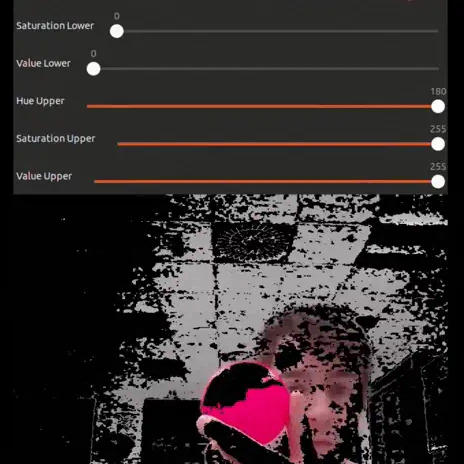
\includegraphics[width=8cm]{figs/opencv_visualization}
  \end{center}
  \caption{\textit{Sliders} de un filtro de color con OpenCV.}
  \label{fig:opencv}
\end{figure}\

Asimismo, se ha utilizado software externo, como
PlotJuggler\footnote{\url{https://plotjuggler.io/}}, para mostrar gráficas sobre
datos provenientes de \textit{topics} en directo.


